\documentclass[12pt]{article} % Default font size is 12pt, it can be changed here
\usepackage[utf8]{inputenc}
\usepackage{geometry} % Required to change the page size to A4
\geometry{a4paper} % Set the page size to be A4 as opposed to the default US Letter
\usepackage{listings}
\usepackage{parskip}
\usepackage{xcolor}
\usepackage{float}
\usepackage{graphicx} % Required for including pictures
\usepackage{hyperref}
\usepackage{float} % Allows putting an [H] in \begin{figure} to specify the exact location of the figure
\usepackage{cite}
\usepackage{fancyhdr}
\usepackage{lscape}
\usepackage{afterpage}

\linespread{1.2} % Line spacing

%\setlength{\parindent}{15pt}
%\setlength\parindent{0pt} % Uncomment to remove all indentation from paragraphs

\graphicspath{{./add/}} % Specifies the directory where pictures are stored

\pagestyle{fancy}
\lhead{Repositorio de árboles genealógicos en BD NoSQL}
\rhead{Daniel Albarral Nuñez}
\cfoot{\thepage}
\renewcommand{\headrulewidth}{0.4pt}
\renewcommand{\footrulewidth}{0.4pt}
\begin{document}

\begin{titlepage}

\newcommand{\HRule}{\rule{\linewidth}{0.5mm}} % Defines a new command for the horizontal lines, change thickness here

\center % Center everything on the page
 
%----------------------------------------------------------------------------------------
%	HEADING SECTIONS
%----------------------------------------------------------------------------------------

\textsc{\LARGE Universidad Politécnica de Cataluña}\\[1.5cm] % Name of your university/college
\textsc{\Large Facultad de Informática de Barcelona}\\[0.5cm] % Major heading such as course name
\textsc{\large Ingeniería de software}\\[0.5cm] % Minor heading such as course 

%----------------------------------------------------------------------------------------
%	TITLE SECTION
%----------------------------------------------------------------------------------------

\HRule \\[0.4cm]
{ \huge \bfseries Repositorio de árboles genealógicos en BD NoSQL}\\[0.4cm] % Title of your document
\HRule \\[1.5cm]
 
%----------------------------------------------------------------------------------------
%	AUTHOR SECTION
%----------------------------------------------------------------------------------------

\begin{minipage}{0.4\textwidth}
\begin{flushleft} \large
\emph{Autor:}\\
Daniel \textsc{Albarral Nuñez} % Your name
\end{flushleft}
\end{minipage}
~
\begin{minipage}{0.4\textwidth}
\begin{flushright} \large
\emph{Supervisor:} \\
Enric \textsc{Mayol} % Supervisor's Name
\end{flushright}
\end{minipage}\\[4cm]

% If you don't want a supervisor, uncomment the two lines below and remove the section above
%\Large \emph{Author:}\\
%John \textsc{Smith}\\[3cm] % Your name

%----------------------------------------------------------------------------------------
%	DATE SECTION
%----------------------------------------------------------------------------------------

{\large Q1 - 2015-2016}\\[2cm] % Date, change the \today to a set date if you want to be precise

%----------------------------------------------------------------------------------------
%	LOGO SECTION
%----------------------------------------------------------------------------------------


\includegraphics[scale=0.7]{logo_upc.png}\\[1cm] % Include a department/university logo - this will require the graphicx package
 
%----------------------------------------------------------------------------------------

\vfill % Fill the rest of the page with whitespace

\end{titlepage}

%----------------------------------------------------------------------------------------
%   TABLE OF CONTENTS
%----------------------------------------------------------------------------------------

\tableofcontents % Include a table of contents

\newpage % Begins the essay on a new page instead of on the same page as the table of contents 

%----------------------------------------------------------------------------------------
%   Contextualización del proyecto
%----------------------------------------------------------------------------------------
\section{Contextualización del proyecto}

\subsubsection{Los arboles genealógicos}
Un arboles genealógico, también llamado genorama, es la representación gráfica de los antepasados  y descendientes de un individuo.Para su representación  se suelen usar tablas o arboles, siendo esta ultima la forma más común y la que se usara en el proyecto.

\subsubsection{Uso y aplicación de los arboles genealógicos.}
Los arboles genealógicos son una herramienta de la genealogía, que se encarga de estudiar y seguir la ascendencia y descendencia de una persona o familia. La genealogía es una ciencia auxiliar de la Historia y es trabajada por un genealogista. Uno de los objetivos del software a desatollar es dar soporte a los genealogistas. \linebreak Por otro lado hay varias comunidades de aficionados que llevan sus propios arboles genealógicos, el software creado también les podrá dar servicio a esta tipología de usuarios.

\newpage
\subsection{Perspectiva general del software actual.}
Todo software genealógico, como mínimo permite almacenar la siguiente información de un individuo: fecha y lugar de nacimiento, fecha de casamiento, muerte y relaciones familiares, contra más flexible es el programa más información te permite introducir acerca de un individuo. También proporcionan diferentes maneras de representar la información y permiten exportar a GEDCOM la información representada.

\noindent\fbox{\parbox{\textwidth}{\begin{flushleft} GEDCOM \cite{aboutGEDCOM} (\textbf{G}enealogical \textbf{D}ata \textbf{COM}munication):\end{flushleft} Es un formato de archivo de datos, proporciona un formato flexible y uniforme para el intercambio de datos genealógicos computarizados.}}

La mayor parte del software genealógico actual esta basado en soluciones de escritorio, pero en los últimos años han proliferado diferentes soluciones web como myheritage o familysearch, que no solo sirven como plataforma de edición sino que también son grandes plataformas \textit{cloud} en las que se almacenan los arboles genealógicos.

Las soluciones más avanzadas, aparte de la gestión de arboles también ofrecen herramientas más orientadas a la investigación, como podrían ser sistemas de búsqueda de individuos basados en sus relaciones o herramientas estadísticas.

\subsection{Tecnología}
Dada la naturaleza social del tipo de software que se busca desarrollar, nacen ciertas complicaciones tecnológicas que en los últimos tiempos se han sido considerablemente investigadas, debido a la gran repercusión de las redes sociales. Las tecnologías clásicas orientadas a la persistencia de datos como las bases de datos SQL, plantean la dificultad de tener un coste muy alto de consulta cuando se pregunta acerca de datos  con un alto nivel de relación entre ellos. Una de las soluciones más usadas para solucionar este problema son las bases de datos basadas en grafos, uno de los casos de éxito es el caso de Twitter, que desarrollo su propia solución, FolckDB, una base de datos basada en grafos, tolerante a fallos, diseñada para tratar con grandes conjuntos de datos, con información no critica.\newline
En el libro \textbf{Neo4j in Action} \cite{neo4jinaction}, Partner and Vukotic realizan el siguiente experimento: \newline
El experimento consiste en comparar una base de datos relacional con neo4j \textit{GraphDB}, en ambas se representa el mismo modelo donde diferentes personas tienen multiples amigos. Se realizan diferentes consultas donde se pretende aberiguar si existe un camino entre dos personas escojidas al azar que los una en una profundidad de como mucho cinco relaciones. Las bases de datos constan de 1000000 personas, cada una con 50 amigos aproximadamente. Los resultados fueron los siguientes:

\begin{figure}[ht!]
\center
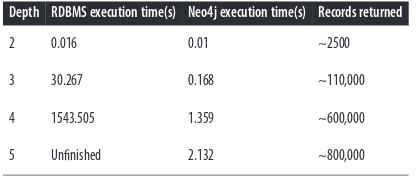
\includegraphics[scale=0.5]{table_find_friends_experiment.png}
\caption{Comparativa entre neo4j y base de datos relacional.}
\label{fig:compa}
\end{figure}

Con este experimento podemos ver como en las consultas donde la profundidad es mayor, o dicho de otra forma, donde la conectividad juega un papel más importante, la base de datos basada en grafos es mucho más rápida. Esto es debido, en gran parte, a que las relaciones en las bases de datos basadas en grafos son \textit{ciudadanos de primer orden} a diferencia de las bases de datos relacionales que tratan las relaciones mediante claves foráneas, lo que proboca que tengan que usar una gran cantidad de joins para resolver el problema, elevando mucho el coste computacional.

\subsubsection{Bases de datos basadas en grafos.}
La gran cantidad de proyectos que han nacido en los últimos años hace prácticamente imposible hacer una comparativa concreta de todas las tecnologías existentes. Pero podemos diferenciar el panorama actual haciendo dos generalizaciones:
\begin{description}
\item[Tecnologías usadas para propósitos transaccionales].\linebreak Orientadas ha dar un servicio online en tiempo real a una aplicación.
\linebreak Estas tecnologías son llamadas \textbf\textit{bases de datos basadas en grafos}. Estas son nuestro principal objeto de estudio. Son el equivalente a las OLTP en el modelo transaccional.
\item[Tecnologías usadas principalmente para el análisis de grafos].\linebreak Llamados \textbf\textit{Motores de procesamiento de grafos}, siguiendo el mismo símil que antes, podríamos pensarlos como herramientas de \textit{data mining} y análisis de procesos(OLAP)
\end{description}

\noindent\fbox{\parbox{\textwidth}{\begin{flushleft} OLTP (\textbf{O}n\textbf{L}ine \textbf{T}ransaction \textbf{P}rocessing):\end{flushleft} Es un tipo de procesamiento que facilita y administra aplicaciones transaccionales, usualmente para entrada de datos y recuperación y procesamiento de transacciones (gestor transaccional). Los paquetes de software para OLTP se basan en la arquitectura cliente-servidor ya que suelen ser utilizados por empresas con una red informática distribuida..}}

Las bases de datos basadas en grafos son sistemas de bases de datos que permiten operaciones CRUD (\textit{Create, Read, Update y Delete}) sobre los objetos representados en ellas. Suelen estar orientadas a funcionar con sistemas transaccionales (OLTP), como aviamos mencionado anteriormente. Sus principales propiedades son, las relaciones son \textit{ciudadanos de primer orden}, a diferencia de otros modelos, como el relacional que tienen que usar claves foráneas. En este tipo de base de datos para representar el dominio de nuestro problema simplemente nos basta con definir los nodos y las relaciones que lo componen.

En el libro Graph Databases \cite{graphdbbook}, encontramos el siguiente gráfico (Figure \ref{fig:grdb}), que nos da una idea de las principales tecnologías basadas en grafos y su orientación.

\begin{figure}[ht!]
\center
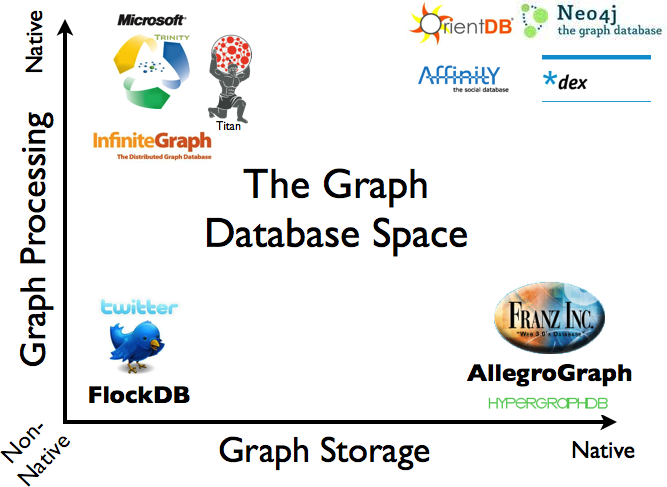
\includegraphics{grdb.png}
\caption{Visión del conjunto de tecnologías}
\label{fig:grdb}
\end{figure}


%----------------------------------------------------------------------------------------
%   Planificación !!PENDIENTE
%----------------------------------------------------------------------------------------
\afterpage{\null\newpage}
\newpage


\section{Planificación}
Para el desarrollo del proyecto se usara \textit{Scrum}, por ello la planificación temporal estará estructurada para facilitar la consecución de esta metodología. El final del proyecto se ha establecido el 22 de abril del 2016.

\subsection{Gantt}
El gantt adjuntado a continuación tiene varias peculiaridades:
\begin{description}
\item [Dependencias de las tareas]. 
\linebreak Dado que en el proyecto se desarrolla íntegramente por una sola persona, la secuencialidad del diagrama es absoluta, por ese motivo también se ha omitido el gráfico PERT.
\item [Fase de desarrollo].
\linebreak Durante la fase de desarrollo simplemente se especifican los \textit{Sprints} que se llevaran a cabo hasta conseguir la consecución del proyecto, a medida que las historias de usuario se vayan redactando y priorizando se irán asignando a los \textit{sprints}.
\end{description}
\newpage

\begin{landscape}

\subsubsection{Tareas}
\begin{figure}[ht!]
\center
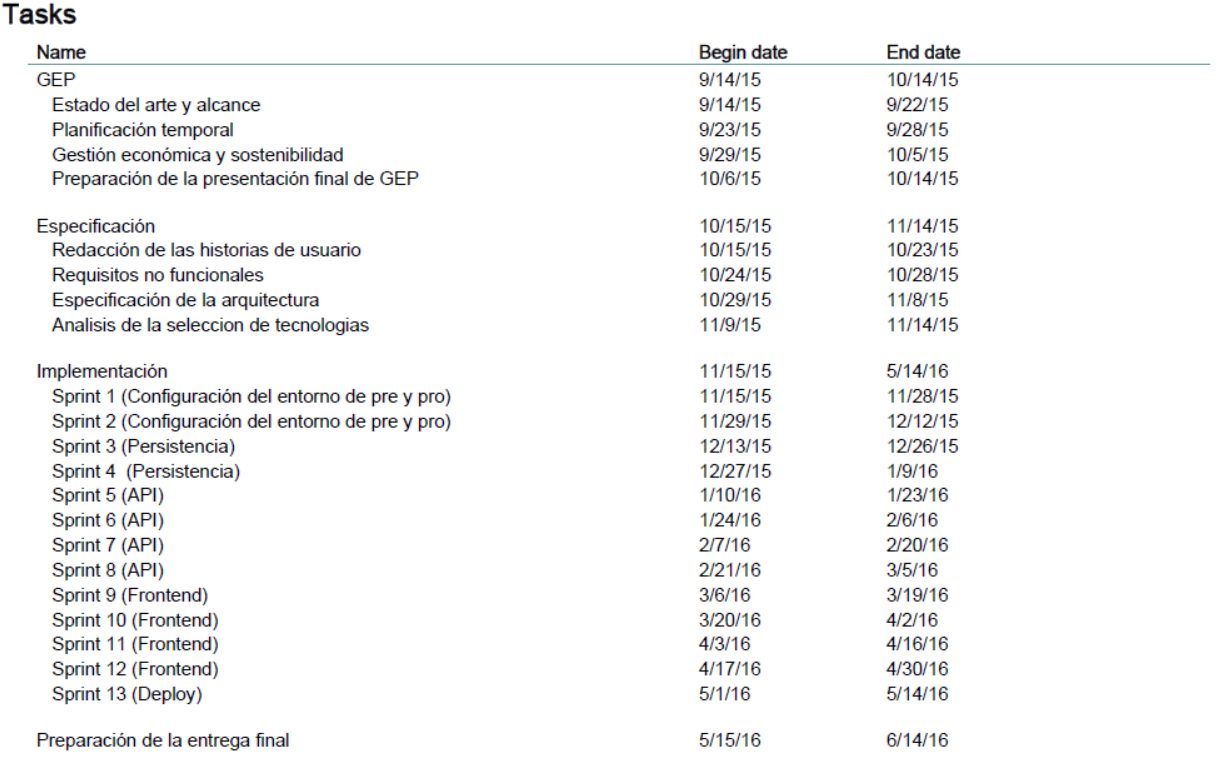
\includegraphics[width=\textwidth,height=\textheight,keepaspectratio]{Task.PNG}
\label{fig:task}
\end{figure}

\newpage
\subsubsection{Gráfico gantt}

\begin{figure}[ht!]
\center
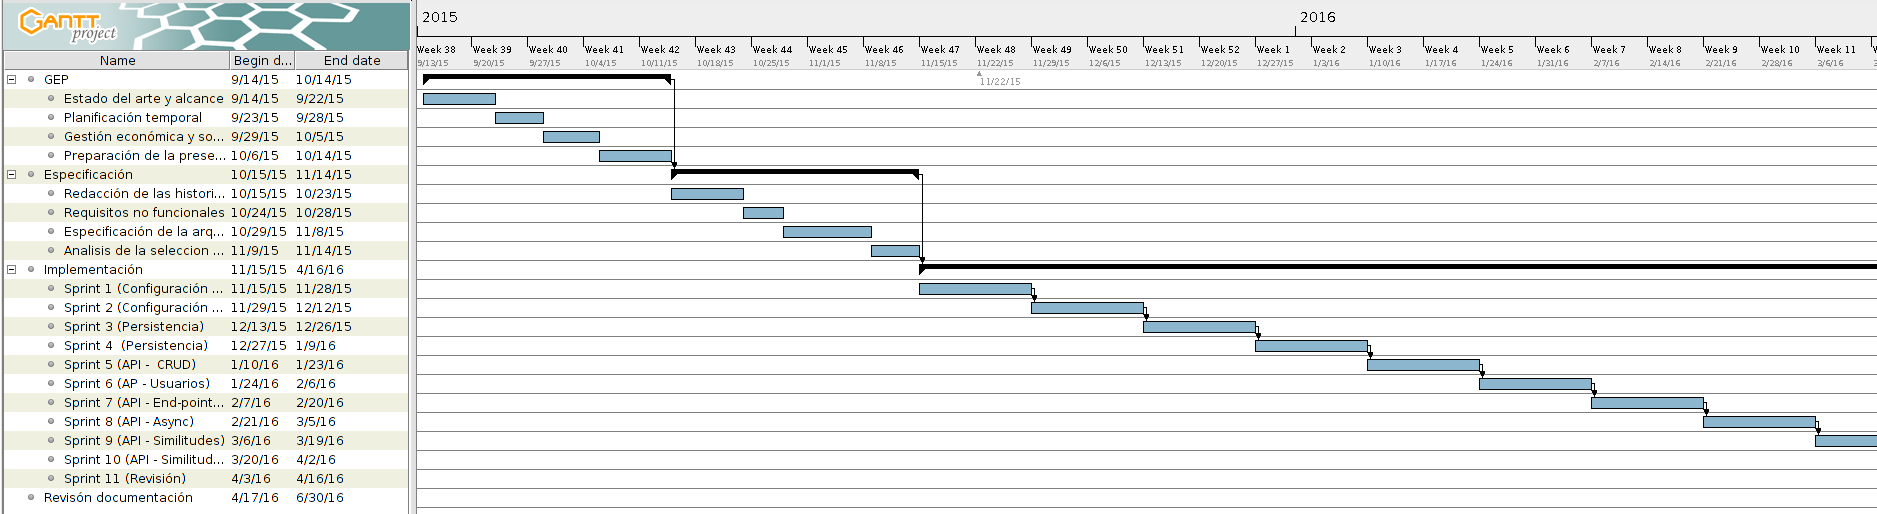
\includegraphics[width=\textwidth,height=\textheight,keepaspectratio]{Gantt_1.PNG}
\label{fig:gantt_1}
\end{figure}

\begin{figure}[ht!]
\center
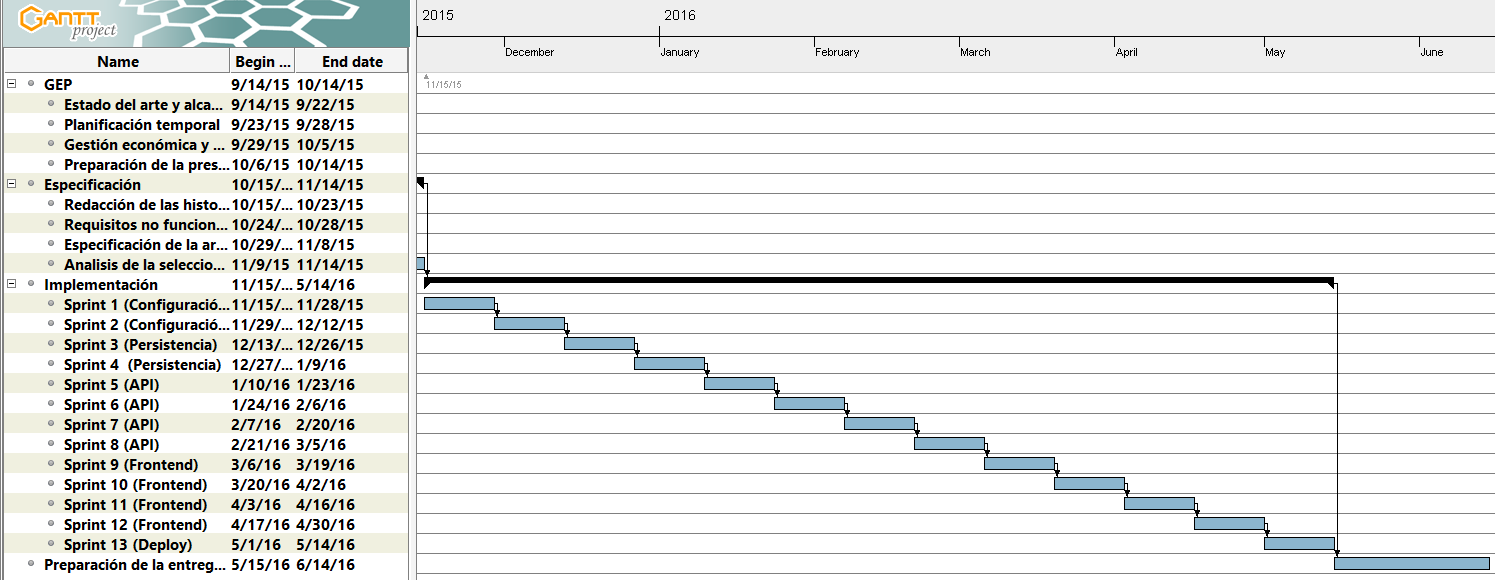
\includegraphics[width=\textwidth,height=\textheight,keepaspectratio]{Gantt_2.PNG}
\label{fig:gantt_2}
\end{figure}

\end{landscape}
\newpage

\subsection{Recursos}
Las necesidades en recursos serán muy escuetas dado que todo el software que se usara es libre y las maquinas en las que se trabaja en preprducción serán virtuales. La única necesidad de tener unos recursos que se necesiten planificar, ya que requieren ser contratados, son los servidores en los que se hará el \textit{deploy}, se tendrán que contratar durante las semanas que dures los \textit{sprints} en los que se haga el \textit{deploy.}

\subsection{Alterativas y plan de acción}
Dado que el proyecto se desarrollara usando \textit{Scrum}, al final de cada \textit{sprint}, durante el \textit{sprint backlog} se determinara si se han  
cumplido las expectativas del \textit{sprint}. Por otro lado en el \textit{sprint planning} se tendrá en cuenta si han habido carencias o bugs en los anteriores \textit{sprints} para incorporarlos como historias de usuario al siguiente \textit{sprint}. 

Como se ha comentado en el alcance, se diseñara un software abierto orientado al desarrollo continuado. Por lo que en el sprint 13 se dará por concluido el proyecto, y se documentara el estado en el que se encuentre y las historias de usuario pendientes.

%----------------------------------------------------------------------------------------
%   Metodolofía y rigor
%----------------------------------------------------------------------------------------
\section{Metodología y rigor}

Las metodologías usadas son las siguientes:

\subsection{SCRUM}
Para el desarrollo del proyecto se ha escojido como metodologia de trabajo SCRUM, los sprints dado la naturaleza del proyecto se han adaptado esta metodologia agil para ser usada por una sola persona. La metodologia de trabajo se ha definido de la siguiente forma:
\begin{description}
	\item[Product backlog]:
	\linebreak Para crear el \textit{product backlog} se han dfinido un seguido de historias de usuario, de acuerdo con el tutor del proyecto, que asume el rol de \textit{product owner}. Estas historias de usuario se revisaran constantemente en los \textit{sprint backlogs}.
	\item[Sprints]:
	\linebreak Los sprints se desarrollaran a lo largo de dos semanas, en este tiempo se desarrollaran las historias de usuario escojidas.
	\item[Sprint backlog]:
	\linebreak Se realizaran al final de cada sprint, dado que esta tarea estara limitada por la disponibilidad del tutor y el alumno, se dara flexibilidad pudiendo realizar el \textit{sprint backlog} de varios sprints en una reunion. 
	\item[Sprint backlog]:
	\linebreak Se realizaran al final de cada sprint, dado que esta tarea estara limitada por la disponibilidad del tutor y el alumno, se dara flexibilidad pudiendo realizar el \textit{sprint backlog} de varios sprints en una reunion. Durante estas reuniones se revisaran las historias de usuario, reorganizando su prioridad, modificando su contenido, añadiendo nuevas o eliminando historias que no se crean necesarias.
\end{description}

%----------------------------------------------------------------------------------------
%   Análisis de alternativas
%----------------------------------------------------------------------------------------
\section{Análisis de alternativas}
%----------------------------------------------------------------------------------------
%   Integración de conocimientos
%----------------------------------------------------------------------------------------
\section{Integración de conocimientos}
%----------------------------------------------------------------------------------------
%   Integración de leyes y regulaciones
%----------------------------------------------------------------------------------------
\section{Integración de leyes y regulaciones}

\newpage

\bibliography{mybibliography}
\nocite{*}
\bibliographystyle{plain}

\end{document}
